\FloatBarrier
\subsection{LS identification with colored noise on output}
We adjusted the Simulink model and MATLAB code from the previous section to incorporate white noise on the output. The output noise amplitude was set to $10\%$ of the system's actual output amplitude. The resulting Simulink model, \autoref{fig:LSICNOSimulinkModel}, represents a system with white noise input and colored noise on the output.

\begin{figure}
	\centering
	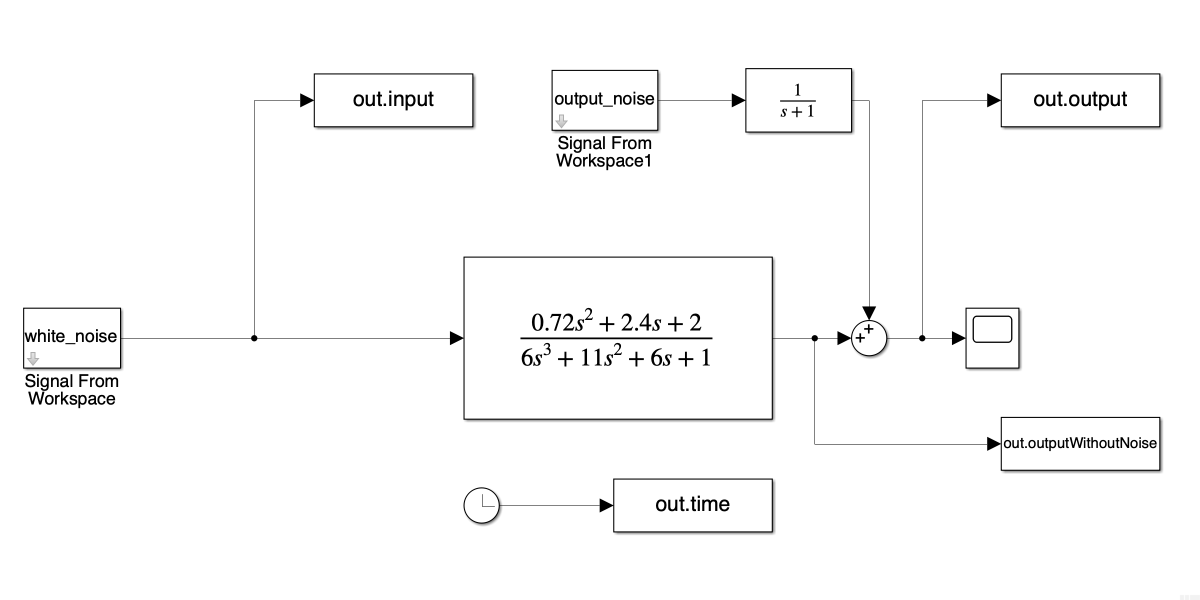
\includegraphics[totalheight=8cm]{images/LSICNOSimulinkModel.png}
	\caption{Simulink model with colored noise on output}
	\label{fig:LSICNOSimulinkModel}
\end{figure}

The identified system's output is compared to the actual system's output (without noise). \autoref{fig:LSICNOOutputVSSimulated} displays this comparison when a white noise input is used.

\begin{figure}
	\centering
	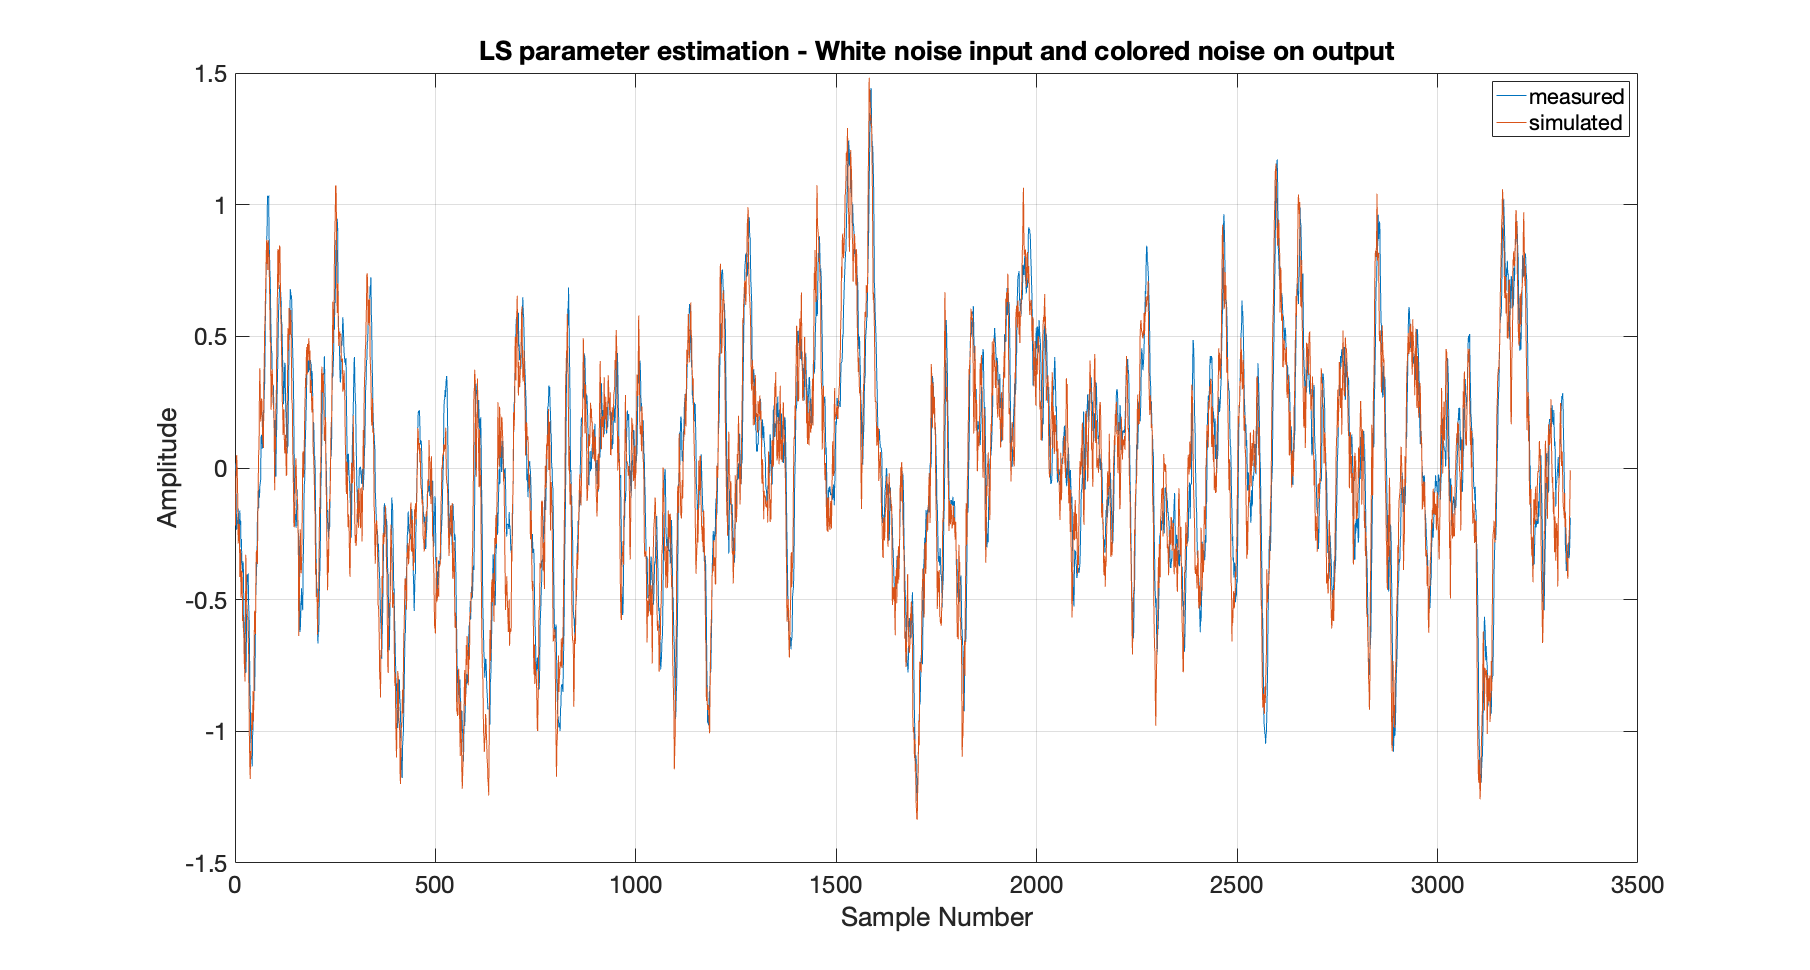
\includegraphics[totalheight=8cm]{images/LSICNOOutputVSSimulated.png}
	\caption{LS system output comparison for colored noise on output}
	\label{fig:LSICNOOutputVSSimulated}
\end{figure}

The Colored noise on the output makes the resulted MSE worse than previous section. The MSE is higher and has a magnitude of $10^{-2}$ (example: 0.0014). \autoref{eq:LSICNONoiseInput} demonstrates the transfer function of the identified system with white noise input.

\begin{equation}
	G(z) =	\frac{0.0428 z^2 + 0.0163 z + 0.01167}{z^3 - 0.9348 z^2 - 0.03248 z + 0.001499}
	\label{eq:LSICNONoiseInput}
\end{equation}


The Simulink model and Matlab code for colored noise on output is located at  \hspace{-1ex}\lstinline| assignment1/part1/1_3/LS1_3_colored.m| and  \hspace{-1ex}\lstinline| assignment1/part1/1_3/LS1_3_clrd.slx|. 
